\documentclass{beamer}

% Should be documentclass beamer

\mode<presentation>
{
%  \usetheme[hideothersubsections]{PaloAlto}
  \usetheme{metropolis}
  \setbeamercovered{transparent}
}

\usepackage{amsfonts}
\usepackage{amsmath}
\usepackage{amssymb}
\usepackage{color}
\usepackage{tikz}
\usepackage{pgfplots}
\usepackage{listings}
\usepackage{courier}
%\usepackage[utf8]{inputenc}
%\usepackage[russian]{babel}

\lstset{
  numbers=left,
  basicstyle=\ttfamily\footnotesize,
  numberstyle=\tiny\color{gray},
  stepnumber=1,
  numbersep=10pt,
}

\newcommand{\iu}{\ensuremath{\mathrm{i}}}
\newcommand{\bbR}{\mathbb{R}}
\newcommand{\bbC}{\mathbb{C}}
\newcommand{\calV}{\mathcal{V}}
\newcommand{\calW}{\mathcal{W}}
\newcommand{\macheps}{\epsilon_{\mathrm{mach}}}
\newcommand{\matlab}{\textsc{Matlab}}

\newcommand{\ddiag}{\operatorname{diag}}
\newcommand{\fl}{\operatorname{fl}}
\newcommand{\nnz}{\operatorname{nnz}}
\newcommand{\tr}{\operatorname{tr}}
\renewcommand{\vec}{\operatorname{vec}}

\newcommand{\vertiii}[1]{{\left\vert\kern-0.25ex\left\vert\kern-0.25ex\left\vert #1
    \right\vert\kern-0.25ex\right\vert\kern-0.25ex\right\vert}}
\newcommand{\ip}[2]{\langle #1, #2 \rangle}
\newcommand{\ipx}[2]{\left\langle #1, #2 \right\rangle}
\newcommand{\order}[1]{O( #1 )}

\newcommand{\kron}{\otimes}


\newcommand{\hdr}[2]{
  \title[CS 5220, Fall 2017]{CS 5220: #2}
  \author{David Bindel}
  \date{#1}
}


\hdr{2017-11-09}{Load Balancing}

\begin{document}

\begin{frame}
  \titlepage
\end{frame}


\begin{frame}
  \frametitle{Inefficiencies in parallel code}

  \begin{center}
    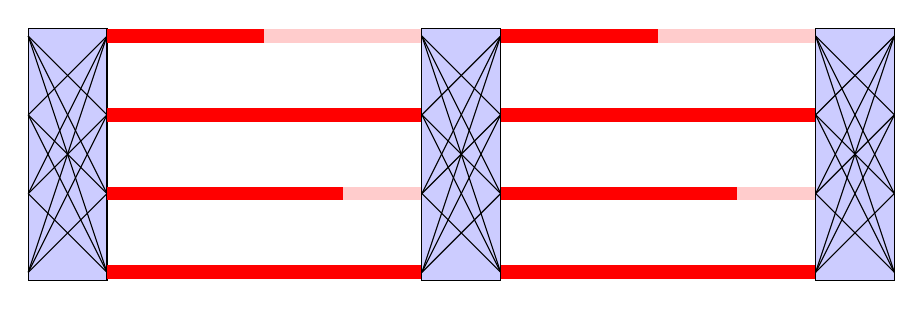
\begin{tikzpicture}

      \begin{scope}[xshift=-1cm]
        \draw[fill=blue!20] (0,-0.1) rectangle (1,3.1);
        \draw (0,0) -- (1,1); \draw (0,0) -- (1,2); \draw (0,0) -- (1,3);
        \draw (0,1) -- (1,0); \draw (0,1) -- (1,2); \draw (0,1) -- (1,3);
        \draw (0,2) -- (1,0); \draw (0,2) -- (1,1); \draw (0,2) -- (1,3);
        \draw (0,3) -- (1,0); \draw (0,3) -- (1,1); \draw (0,3) -- (1,2);
      \end{scope}
      
      \begin{scope}
        \draw[line width=5pt, red]    (0,0) -- (4,0);
        \draw[line width=5pt, red]    (0,1) -- (3,1);
        \draw[line width=5pt, red!20] (3,1) -- (4,1);
        \draw[line width=5pt, red]    (0,2) -- (4,2);
        \draw[line width=5pt, red]    (0,3) -- (2,3);
        \draw[line width=5pt, red!20] (2,3) -- (4,3);
      \end{scope}

      \begin{scope}[xshift=4cm]
        \draw[fill=blue!20] (0,-0.1) rectangle (1,3.1);
        \draw (0,0) -- (1,1); \draw (0,0) -- (1,2); \draw (0,0) -- (1,3);
        \draw (0,1) -- (1,0); \draw (0,1) -- (1,2); \draw (0,1) -- (1,3);
        \draw (0,2) -- (1,0); \draw (0,2) -- (1,1); \draw (0,2) -- (1,3);
        \draw (0,3) -- (1,0); \draw (0,3) -- (1,1); \draw (0,3) -- (1,2);
      \end{scope}
      
      \begin{scope}[xshift=5cm]
        \draw[line width=5pt, red]    (0,0) -- (4,0);
        \draw[line width=5pt, red]    (0,1) -- (3,1);
        \draw[line width=5pt, red!20] (3,1) -- (4,1);
        \draw[line width=5pt, red]    (0,2) -- (4,2);
        \draw[line width=5pt, red]    (0,3) -- (2,3);
        \draw[line width=5pt, red!20] (2,3) -- (4,3);
      \end{scope}

      \begin{scope}[xshift=9cm]
        \draw[fill=blue!20] (0,-0.1) rectangle (1,3.1);
        \draw (0,0) -- (1,1); \draw (0,0) -- (1,2); \draw (0,0) -- (1,3);
        \draw (0,1) -- (1,0); \draw (0,1) -- (1,2); \draw (0,1) -- (1,3);
        \draw (0,2) -- (1,0); \draw (0,2) -- (1,1); \draw (0,2) -- (1,3);
        \draw (0,3) -- (1,0); \draw (0,3) -- (1,1); \draw (0,3) -- (1,2);
      \end{scope}
      
    \end{tikzpicture}
  \end{center}
  
  Poor single processor performance
  \begin{itemize}
    \item Typically in the memory system
    \item Saw this in matrix multiply assignment
  \end{itemize}
\end{frame}


\begin{frame}
  \frametitle{Inefficiencies in parallel code}

  \begin{center}
    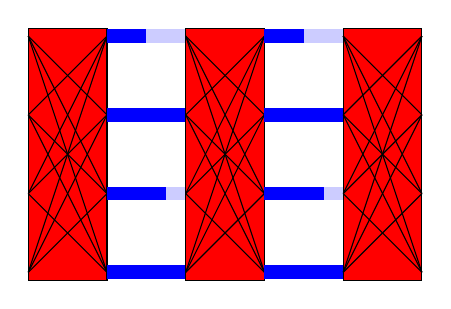
\begin{tikzpicture}

      \begin{scope}[xshift=-1cm]
        \draw[fill=red] (0,-0.1) rectangle (1,3.1);
        \draw (0,0) -- (1,1); \draw (0,0) -- (1,2); \draw (0,0) -- (1,3);
        \draw (0,1) -- (1,0); \draw (0,1) -- (1,2); \draw (0,1) -- (1,3);
        \draw (0,2) -- (1,0); \draw (0,2) -- (1,1); \draw (0,2) -- (1,3);
        \draw (0,3) -- (1,0); \draw (0,3) -- (1,1); \draw (0,3) -- (1,2);
      \end{scope}
      
      \begin{scope}[xscale=0.25]
        \draw[line width=5pt, blue]    (0,0) -- (4,0);
        \draw[line width=5pt, blue]    (0,1) -- (3,1);
        \draw[line width=5pt, blue!20] (3,1) -- (4,1);
        \draw[line width=5pt, blue]    (0,2) -- (4,2);
        \draw[line width=5pt, blue]    (0,3) -- (2,3);
        \draw[line width=5pt, blue!20] (2,3) -- (4,3);
      \end{scope}

      \begin{scope}[xshift=1cm]
        \draw[fill=red] (0,-0.1) rectangle (1,3.1);
        \draw (0,0) -- (1,1); \draw (0,0) -- (1,2); \draw (0,0) -- (1,3);
        \draw (0,1) -- (1,0); \draw (0,1) -- (1,2); \draw (0,1) -- (1,3);
        \draw (0,2) -- (1,0); \draw (0,2) -- (1,1); \draw (0,2) -- (1,3);
        \draw (0,3) -- (1,0); \draw (0,3) -- (1,1); \draw (0,3) -- (1,2);
      \end{scope}
      
      \begin{scope}[xshift=2cm,xscale=0.25]
        \draw[line width=5pt, blue]    (0,0) -- (4,0);
        \draw[line width=5pt, blue]    (0,1) -- (3,1);
        \draw[line width=5pt, blue!20] (3,1) -- (4,1);
        \draw[line width=5pt, blue]    (0,2) -- (4,2);
        \draw[line width=5pt, blue]    (0,3) -- (2,3);
        \draw[line width=5pt, blue!20] (2,3) -- (4,3);
      \end{scope}

      \begin{scope}[xshift=3cm]
        \draw[fill=red] (0,-0.1) rectangle (1,3.1);
        \draw (0,0) -- (1,1); \draw (0,0) -- (1,2); \draw (0,0) -- (1,3);
        \draw (0,1) -- (1,0); \draw (0,1) -- (1,2); \draw (0,1) -- (1,3);
        \draw (0,2) -- (1,0); \draw (0,2) -- (1,1); \draw (0,2) -- (1,3);
        \draw (0,3) -- (1,0); \draw (0,3) -- (1,1); \draw (0,3) -- (1,2);
      \end{scope}
      
    \end{tikzpicture}
  \end{center}
  
  Overhead for parallelism
  \begin{itemize}
    \item Thread creation, synchronization, communication
    \item Saw this in moshpit and shallow water assignments
  \end{itemize}
\end{frame}


\begin{frame}
  \frametitle{Inefficiencies in parallel code}

  \begin{center}
    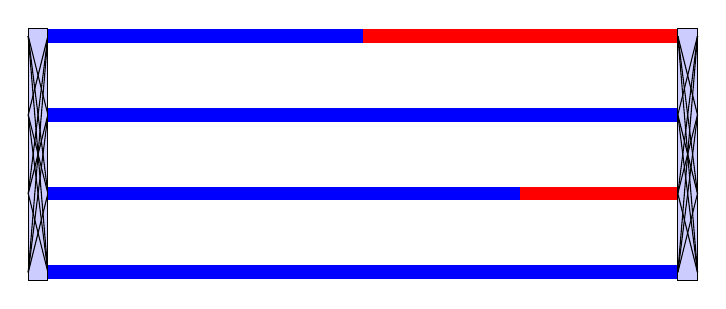
\begin{tikzpicture}

      \begin{scope}[xshift=-0.25cm,xscale=0.25]
        \draw[fill=blue!20] (0,-0.1) rectangle (1,3.1);
        \draw (0,0) -- (1,1); \draw (0,0) -- (1,2); \draw (0,0) -- (1,3);
        \draw (0,1) -- (1,0); \draw (0,1) -- (1,2); \draw (0,1) -- (1,3);
        \draw (0,2) -- (1,0); \draw (0,2) -- (1,1); \draw (0,2) -- (1,3);
        \draw (0,3) -- (1,0); \draw (0,3) -- (1,1); \draw (0,3) -- (1,2);
      \end{scope}
      
      \begin{scope}[xscale=2]
        \draw[line width=5pt, blue]    (0,0) -- (4,0);
        \draw[line width=5pt, blue]    (0,1) -- (3,1);
        \draw[line width=5pt, red]     (3,1) -- (4,1);
        \draw[line width=5pt, blue]    (0,2) -- (4,2);
        \draw[line width=5pt, blue]    (0,3) -- (2,3);
        \draw[line width=5pt, red]     (2,3) -- (4,3);
      \end{scope}

      \begin{scope}[xshift=8cm,xscale=0.25]
        \draw[fill=blue!20] (0,-0.1) rectangle (1,3.1);
        \draw (0,0) -- (1,1); \draw (0,0) -- (1,2); \draw (0,0) -- (1,3);
        \draw (0,1) -- (1,0); \draw (0,1) -- (1,2); \draw (0,1) -- (1,3);
        \draw (0,2) -- (1,0); \draw (0,2) -- (1,1); \draw (0,2) -- (1,3);
        \draw (0,3) -- (1,0); \draw (0,3) -- (1,1); \draw (0,3) -- (1,2);
      \end{scope}
            
    \end{tikzpicture}
  \end{center}
  
  Load imbalance
  \begin{itemize}
    \item Different amounts of work across processors
    \item Different speeds / available resources
    \item Insufficient parallel work
    \item All this can change over phases
  \end{itemize}
\end{frame}


\begin{frame}
  \frametitle{Where does the time go?}

  \begin{itemize}
  \item
    Load balance looks like large sync cost
  \item
    ... maybe so does ordinary synchronization overhead!
  \item
    And spin-locks may make sync look like useful work
  \item
    And ordinary time sharing can confuse things more
  \item
    Can get some help from profiling tools
  \end{itemize}
\end{frame}


\begin{frame}
  \frametitle{Many independent tasks}
  
  \begin{center}
    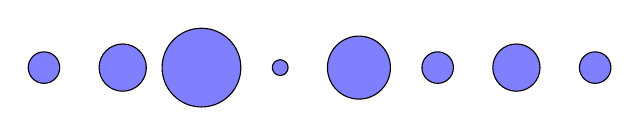
\begin{tikzpicture}
      \draw[fill=blue!50] (0,0) circle (2mm);
      \draw[fill=blue!50] (1,0) circle (3mm);
      \draw[fill=blue!50] (2,0) circle (5mm);
      \draw[fill=blue!50] (3,0) circle (1mm);
      \draw[fill=blue!50] (4,0) circle (4mm);
      \draw[fill=blue!50] (5,0) circle (2mm);
      \draw[fill=blue!50] (6,0) circle (3mm);
      \draw[fill=blue!50] (7,0) circle (2mm);
    \end{tikzpicture}
  \end{center}

  \begin{itemize}
  \item Simplest strategy: partition by task index
    \begin{itemize}
    \item What if task costs are inhomogeneous?
    \item Worse: what if expensive tasks all land on one thread?
    \end{itemize}
  \item Potential fixes
    \begin{itemize}
    \item Many small tasks, randomly assigned to processors
    \item Dynamic task assignment
    \end{itemize}
  \item Issue: what about scheduling overhead?
  \end{itemize}
\end{frame}
  
\begin{frame}
  \frametitle{Variations on a theme}

  How to avoid overhead?  Chunks!  (Think OpenMP loops)
  \begin{itemize}
  \item Small chunks: good balance, large overhead
  \item Large chunks: poor balance, low overhead
  \end{itemize}
  Variants:
    \begin{itemize}
    \item Fixed chunk size (requires good cost estimates)
    \item Guided self-scheduling (take $\lceil (\mbox{tasks left})/p \rceil$ work)
    \item Tapering (size chunks based on variance)
    \item Weighted factoring (GSS with heterogeneity)
    \end{itemize}
\end{frame}


\begin{frame}
  \frametitle{Static dependency and graph partitioning}

  \begin{center}
    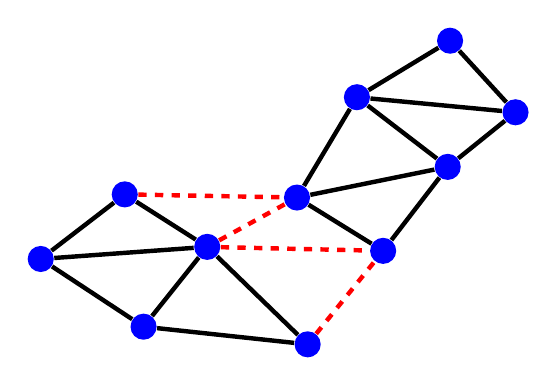
\begin{tikzpicture}
      \node (n1) at (1.108060,0.168294) [circle,fill=blue] {};
\node (n2) at (1.916771,1.181859) [circle,fill=blue] {};
\node (n3) at (-0.197998,1.028224) [circle,fill=blue] {};
\node (n4) at (0.869271,1.848640) [circle,fill=blue] {};
\node (n5) at (3.056732,1.808215) [circle,fill=blue] {};
\node (n6) at (3.192034,-0.055883) [circle,fill=blue] {};
\node (n7) at (4.150780,1.131397) [circle,fill=blue] {};
\node (n8) at (4.970900,2.197872) [circle,fill=blue] {};
\node (n9) at (3.817774,3.082424) [circle,fill=blue] {};
\node (n10) at (5.832186,2.891196) [circle,fill=blue] {};
\node (n11) at (5.000885,3.800002) [circle,fill=blue] {};
\draw[    ultra thick       ] (n1) -- (n2);
\draw[    ultra thick       ] (n1) -- (n3);
\draw[    ultra thick       ] (n1) -- (n6);
\draw[    ultra thick       ] (n2) -- (n3);
\draw[    ultra thick       ] (n2) -- (n4);
\draw[red,ultra thick,dashed] (n2) -- (n5);
\draw[    ultra thick       ] (n2) -- (n6);
\draw[red,ultra thick,dashed] (n2) -- (n7);
\draw[    ultra thick       ] (n3) -- (n4);
\draw[red,ultra thick,dashed] (n4) -- (n5);
\draw[    ultra thick       ] (n5) -- (n7);
\draw[    ultra thick       ] (n5) -- (n8);
\draw[    ultra thick       ] (n5) -- (n9);
\draw[red,ultra thick,dashed] (n6) -- (n7);
\draw[    ultra thick       ] (n7) -- (n8);
\draw[    ultra thick       ] (n8) -- (n9);
\draw[    ultra thick       ] (n8) -- (n10);
\draw[    ultra thick       ] (n9) -- (n10);
\draw[    ultra thick       ] (n9) -- (n11);
\draw[    ultra thick       ] (n10) -- (n11);

    \end{tikzpicture}
  \end{center}
    
  \begin{itemize}
  \item Graph $G = (V,E)$ with vertex and edge weights
  \item Goal: even partition with small edge cut (comm volume)
  \item Optimal partitioning is NP complete -- use heuristics
  \item Tradeoff quality vs speed
  \item Good software exists (e.g. METIS)
  \end{itemize}
\end{frame}


\begin{frame}
  \frametitle{The limits of graph partitioning}

  What if 
  \begin{itemize}
  \item We don't know task costs?
  \item We don't know the communication/dependency pattern?
  \item These things change over time?
  \end{itemize}
  May want {\em dynamic} load balancing?

  \vspace{5mm}
  Even in regular case: not every problem looks like an undirected graph!

\end{frame}


\begin{frame}
  \frametitle{Dependency graphs}

  So far: Graphs for dependencies between {\em unknowns}.
  
  \vspace{5mm}
  For dependency between tasks or computations:
  \begin{itemize}
  \item Arrow from $A$ to $B$ means that $B$ depends on $A$
  \item Result is a {\em directed acyclic graph} (DAG)
  \end{itemize}
\end{frame}


\begin{frame}
  \frametitle{Example: Longest Common Substring}

  Goal: Longest sequence of (not necessarily contiguous) characters
  common to strings $S$ and $T$.

  Recursive formulation:
  \[
  \mathrm{LCS}[i,j] =
  \begin{cases}
    \max(\mathrm{LCS}[i-1,j], \mathrm{LCS}[j,i-1]), & S[i] \neq T[j] \\
    1 + \mathrm{LCS}[i-1,j-1], & S[i] = T[j]
  \end{cases}
  \]
  Dynamic programming: Form a table of $\mathrm{LCS}[i,j]$
\end{frame}


\begin{frame}
  \frametitle{Dependency graphs}

  \begin{center}
  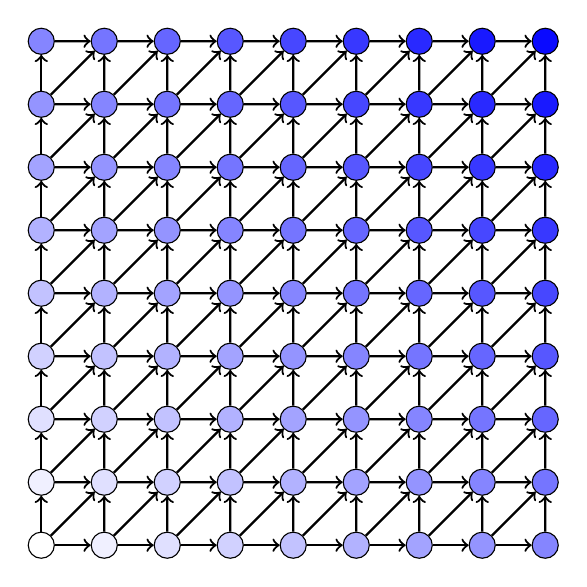
\begin{tikzpicture}[scale=0.8]
    \foreach \x in {0,...,8}
    \foreach \y in {0,...,8} {
        \pgfmathtruncatemacro{\cur}{6*(\x+\y)}
        \node (\x\y) at (\x, \y) [circle,draw=black,fill=blue!\cur] {};
        }
    
      \foreach \x [count=\xp] in {0,...,7}
        \foreach \y in {0,...,8}
        {
          \draw[thick,->] (\x\y) -- (\xp\y);
          \draw[thick,->] (\y\x) -- (\y\xp);
        }
      \foreach \x [count=\xp] in {0,...,7}
        \foreach \y [count=\yp] in {0,...,7}
        {
          \draw[thick,->] (\x\y) -- (\xp\yp);
        }
  \end{tikzpicture} \\
  Can process in any order consistent with dependencies. \\
  Limits to available parallel work early on or late!
  \end{center}
\end{frame}


\begin{frame}
  \frametitle{Dependency graphs}

  \begin{center}
  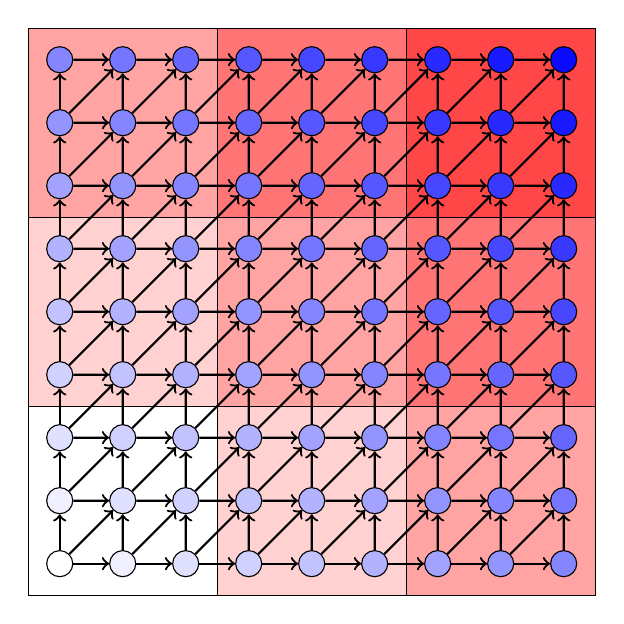
\begin{tikzpicture}[scale=0.8]
    \foreach \x [count=\xp] in {0,...,2}
      \foreach \y [count=\yp] in {0,...,2}
      {
        \pgfmathtruncatemacro{\cur}{18*(\x+\y)}                   
        \draw[fill=red!\cur] (3*\x-0.5,3*\y-0.5) rectangle (3*\xp-0.5,3*\yp-0.5);
      }
      
    \foreach \x in {0,...,8}
    \foreach \y in {0,...,8} {
        \pgfmathtruncatemacro{\cur}{6*(\x+\y)}
        \node (\x\y) at (\x, \y) [circle,draw=black,fill=blue!\cur] {};
        }
    
      \foreach \x [count=\xp] in {0,...,7}
        \foreach \y in {0,...,8}
        {
          \draw[thick,->] (\x\y) -- (\xp\y);
          \draw[thick,->] (\y\x) -- (\y\xp);
        }
      \foreach \x [count=\xp] in {0,...,7}
        \foreach \y [count=\yp] in {0,...,7}
        {
          \draw[thick,->] (\x\y) -- (\xp\yp);
        }

  \end{tikzpicture} \\
  Partition into coarser-grain tasks for locality?
  \end{center}
\end{frame}


\begin{frame}
  \frametitle{Dependency graphs}

  \begin{center}
  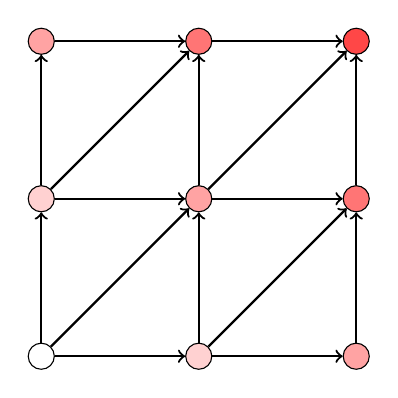
\begin{tikzpicture}[scale=2]
      
    \foreach \x in {0,...,2}
    \foreach \y in {0,...,2} {
        \pgfmathtruncatemacro{\cur}{18*(\x+\y)}
        \node (\x\y) at (\x, \y) [circle,draw=black,fill=red!\cur] {};
        }
    
      \foreach \x [count=\xp] in {0,...,1}
        \foreach \y in {0,...,2}
        {
          \draw[thick,->] (\x\y) -- (\xp\y);
          \draw[thick,->] (\y\x) -- (\y\xp);
        }
      \foreach \x [count=\xp] in {0,...,1}
        \foreach \y [count=\yp] in {0,...,1}
        {
          \draw[thick,->] (\x\y) -- (\xp\yp);
        }

  \end{tikzpicture} \\
  Dependence between coarse tasks limits parallelism.
  \end{center}
\end{frame}


\begin{frame}
  \frametitle{Alternate perspective}

  Recall LCS
  \[
  \mathrm{LCS}[i,j] =
  \begin{cases}
    \max(\mathrm{LCS}[i-1,j], \mathrm{LCS}[j,i-1]), & S[i] \neq T[j] \\
    1 + \mathrm{LCS}[i-1,j-1], & S[i] = T[j]
  \end{cases}
  \]
  Two approaches to LCS:
  \begin{itemize}
  \item Solve subproblems from bottom up
  \item Solve from top down and {\em memoize} common subproblems
  \end{itemize}
  Parallel question: shared memoization (and synchronize) or
  independent memoization (and redundant computation)?
\end{frame}


\begin{frame}
  \frametitle{Load balancing and task-based parallelism}

  \begin{center}
    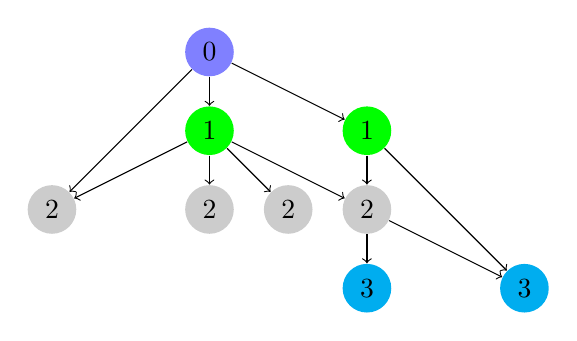
\begin{tikzpicture}
      \node (n0) at (-1,0) [circle,fill=blue!50] {$0$};
      \node (n1) at (-1,-1) [circle,fill=green] {$1$};
      \node (n2) at ( 1,-1) [circle,fill=green] {$1$};
      \node (n3) at (-3,-2) [circle,fill=black!20] {$2$};
      \node (n4) at (-1,-2) [circle,fill=black!20] {$2$};
      \node (n5) at ( 0,-2) [circle,fill=black!20] {$2$};
      \node (n6) at ( 1,-2) [circle,fill=black!20] {$2$};
      \node (n7) at ( 1,-3) [circle,fill=cyan] {$3$};
      \node (n8) at ( 3,-3) [circle,fill=cyan] {$3$};
      \draw[->] (n0) -- (n1);
      \draw[->] (n0) -- (n2);
      \draw[->] (n0) -- (n3);
      \draw[->] (n1) -- (n3);
      \draw[->] (n1) -- (n4);
      \draw[->] (n1) -- (n5);
      \draw[->] (n1) -- (n6);
      \draw[->] (n2) -- (n6);
      \draw[->] (n6) -- (n7);
      \draw[->] (n6) -- (n8);
      \draw[->] (n2) -- (n8);
    \end{tikzpicture}

    \begin{itemize}
    \item Task DAG captures data dependencies
    \item May be known at outset or dynamically generated
    \item Topological sort reveals parallelism opportunities
    \end{itemize}
  \end{center}
\end{frame}


\begin{frame}
  \frametitle{Basic parameters}
  
  \begin{itemize}
  \item Task costs
    \begin{itemize}
    \item Do all tasks have equal costs?
    \item Costs known statically, at creation, at completion?
    \end{itemize}
  \item Task dependencies
    \begin{itemize}
    \item Can tasks be run in any order?
    \item If not, when are dependencies known?
    \end{itemize}
  \item Locality
    \begin{itemize}
    \item Should tasks be co-located to reduce communication?
    \item When is this information known?
    \end{itemize}
  \end{itemize}
\end{frame}


\begin{frame}
  \frametitle{Task costs}

  \begin{center}
    
\begin{tikzpicture}
      \draw[fill=blue!50] (0,0) circle (2mm);
      \draw[fill=blue!50] (1,0) circle (2mm);
      \draw[fill=blue!50] (2,0) circle (2mm);
      \draw[fill=blue!50] (3,0) circle (2mm);
      \draw[fill=blue!50] (4,0) circle (2mm);
      \draw[fill=blue!50] (5,0) circle (2mm);
      \draw[fill=blue!50] (6,0) circle (2mm);
      \draw[fill=blue!50] (7,0) circle (2mm);
    \end{tikzpicture} \\
    Easy: equal unit cost tasks (branch-free loops)
  \end{center}

  \begin{center}
    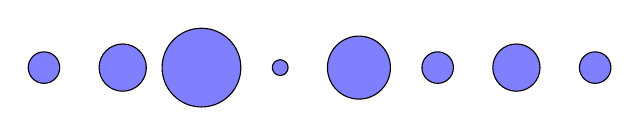
\begin{tikzpicture}
      \draw[fill=blue!50] (0,0) circle (2mm);
      \draw[fill=blue!50] (1,0) circle (3mm);
      \draw[fill=blue!50] (2,0) circle (5mm);
      \draw[fill=blue!50] (3,0) circle (1mm);
      \draw[fill=blue!50] (4,0) circle (4mm);
      \draw[fill=blue!50] (5,0) circle (2mm);
      \draw[fill=blue!50] (6,0) circle (3mm);
      \draw[fill=blue!50] (7,0) circle (2mm);
    \end{tikzpicture} \\
    Harder: different, known times (sparse MVM)
  \end{center}

  \begin{center}
    
\begin{tikzpicture}
      \node at (0,0) [circle,fill=blue!20] {?};
      \node at (1,0) [circle,fill=blue!20] {?};
      \node at (2,0) [circle,fill=blue!20] {?};
      \node at (3,0) [circle,fill=blue!20] {?};
      \node at (4,0) [circle,fill=blue!20] {?};
      \node at (5,0) [circle,fill=blue!20] {?};
      \node at (6,0) [circle,fill=blue!20] {?};
      \node at (7,0) [circle,fill=blue!20] {?};
    \end{tikzpicture} \\
    Hardest: costs unknown until completed (search)
  \end{center}

\end{frame}


\begin{frame}
  \frametitle{Dependencies}

  \begin{center}
    
\begin{tikzpicture}
      \node at (0,0) [circle,fill=blue!50] {};
      \node at (1,0) [circle,fill=blue!50] {};
      \node at (2,0) [circle,fill=blue!50] {};
      \node at (3,0) [circle,fill=blue!50] {};
      \node at (4,0) [circle,fill=blue!50] {};
      \node at (5,0) [circle,fill=blue!50] {};
      \node at (6,0) [circle,fill=blue!50] {};
      \node at (7,0) [circle,fill=blue!50] {};
    \end{tikzpicture} \\
    Easy: dependency-free loop (Jacobi sweep)
  \end{center}

  \begin{center}
    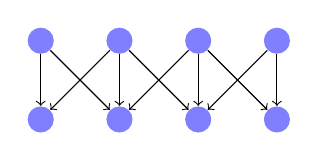
\begin{tikzpicture}
      \node(a0) at (0,0) [circle,fill=blue!50] {};
      \node(a1) at (1,0) [circle,fill=blue!50] {};
      \node(a2) at (2,0) [circle,fill=blue!50] {};
      \node(a3) at (3,0) [circle,fill=blue!50] {};
      \node(b0) at (0,1) [circle,fill=blue!50] {};
      \node(b1) at (1,1) [circle,fill=blue!50] {};
      \node(b2) at (2,1) [circle,fill=blue!50] {};
      \node(b3) at (3,1) [circle,fill=blue!50] {};
      \draw[->] (b0) -- (a0); \draw[->] (b0) -- (a1);
      \draw[->] (b1) -- (a1); \draw[->] (b1) -- (a0); \draw[->] (b1) -- (a2);
      \draw[->] (b2) -- (a2); \draw[->] (b2) -- (a1); \draw[->] (b2) -- (a3);
      \draw[->] (b3) -- (a3); \draw[->] (b3) -- (a2);
    \end{tikzpicture} \\
    Harder: tasks have predictable structure (some DAG)
  \end{center}

  \begin{center}
    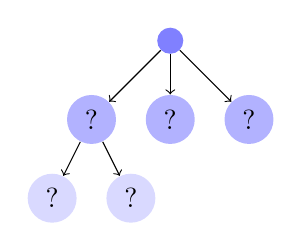
\begin{tikzpicture}
      \node(n0) at (0,2) [circle,fill=blue!50] {};
      \node(n1) at (-1,1) [circle,fill=blue!30] {?};
      \node(n2) at ( 0,1) [circle,fill=blue!30] {?};
      \node(n3) at ( 1,1) [circle,fill=blue!30] {?};
      \node(n4) at (-1.5,0) [circle,fill=blue!15] {?};
      \node(n5) at (-0.5,0) [circle,fill=blue!15] {?};
      \draw[->] (n0) -- (n1);
      \draw[->] (n0) -- (n2);
      \draw[->] (n0) -- (n3);
      \draw[->] (n1) -- (n4);
      \draw[->] (n1) -- (n5);
    \end{tikzpicture} \\
    Hardest: structure is dynamic (search, sparse LU)    
  \end{center}
  
%  \begin{itemize}
%  \item Easy: dependency-free loop (Jacobi sweep)
%  \item Harder: tasks have predictable structure (some DAG)
%  \item Hardest: structure is dynamic (search, sparse LU)
%  \end{itemize}
\end{frame}


\begin{frame}
  \frametitle{Locality/communication}

  When do you communicate?
  \begin{itemize}
  \item Easy: Only at start/end 
    (embarrassingly parallel)
  \item Harder: In a predictable pattern
    (elliptic PDE solver)
  \item Hardest: Unpredictable
    (discrete event simulation)
  \end{itemize}
\end{frame}


\begin{frame}
  \frametitle{A spectrum of solutions}

  How much we can do depends on cost, dependency, locality
  \begin{itemize}
  \item Static scheduling
    \begin{itemize}
    \item Everything known in advance
    \item Can schedule offline (e.g. graph partitioning)
    \item Example: Shallow water solver
    \end{itemize}
  \item Semi-static scheduling
    \begin{itemize}
    \item Everything known at start of step (for example)
    \item Can use offline ideas (e.g. Kernighan-Lin refinement)
    \item Example: Particle-based methods
    \end{itemize}
  \item Dynamic scheduling
    \begin{itemize}
    \item Don't know what we're doing until we've started
    \item Have to use online algorithms
    \item Example: most search problems
    \end{itemize}
  \end{itemize}
\end{frame}


\begin{frame}
  \frametitle{Search problems}

  \begin{itemize}
  \item Different set of strategies from physics sims!
  \item Usually require dynamic load balance
  \item Example:
    \begin{itemize}
    \item Optimal VLSI layout
    \item Robot motion planning
    \item Game playing
    \item Speech processing
    \item Reconstructing phylogeny
    \item ...
    \end{itemize}
  \end{itemize}
\end{frame}


\begin{frame}
  \frametitle{Example: Tree search}

  \begin{center}
    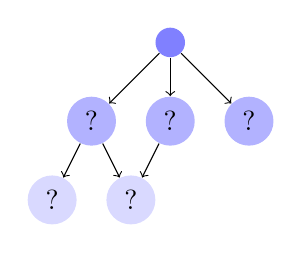
\begin{tikzpicture}
      \node(n0) at (0,2) [circle,fill=blue!50] {\,};
      \node(n1) at (-1,1) [circle,fill=blue!30] {?};
      \node(n2) at ( 0,1) [circle,fill=blue!30] {?};
      \node(n3) at ( 1,1) [circle,fill=blue!30] {?};
      \node(n4) at (-1.5,0) [circle,fill=blue!15] {?};
      \node(n5) at (-0.5,0) [circle,fill=blue!15] {?};
      \draw[->] (n0) -- (n1);
      \draw[->] (n0) -- (n2);
      \draw[->] (n0) -- (n3);
      \draw[->] (n1) -- (n4);
      \draw[->] (n1) -- (n5);
      \draw[->] (n2) -- (n5);
    \end{tikzpicture}
  \end{center}
  \begin{itemize}
  \item Tree unfolds dynamically during search
  \item May be common problems on different paths (graph)
  \item Graph may or may not be explicit in advance
  \end{itemize}
\end{frame}


\begin{frame}
  \frametitle{Search algorithms}

  Generic search:
  \begin{tabbing}
    \quad \= \quad \= \kill
    Put root in stack/queue \\
    while stack/queue has work \\
    \> remove node $n$ from queue \\
    \> if $n$ satisfies goal, return \\
    \> mark $n$ as searched \\
    \> add viable unsearched children of $n$ to stack/queue \\
    \>\> (Can branch-and-bound)
  \end{tabbing}
  Variants: DFS (stack), BFS (queue), A$^*$ (priority queue), ...
\end{frame}


\begin{frame}
  \frametitle{Simple parallel search}

  \begin{center}
    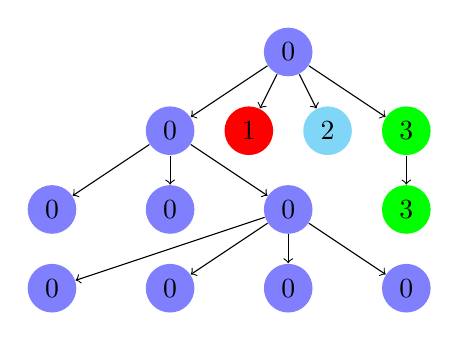
\begin{tikzpicture}
      \node (n0) at (0,5) [circle,fill=blue!50] {0};
      \node (n1) at (-1.5,4) [circle,fill=blue!50]  {0};
      \node (n2) at (-0.5,4) [circle,fill=red]   {1};
      \node (n3) at ( 0.5,4) [circle,fill=cyan!50]  {2};
      \node (n4) at ( 1.5,4) [circle,fill=green] {3};
      \node (n5) at (-3.0,3) [circle,fill=blue!50]  {0};
      \node (n6) at (-1.5,3) [circle,fill=blue!50]  {0};
      \node (n7) at ( 0.0,3) [circle,fill=blue!50]  {0};
      \node (n8) at ( 1.5,3) [circle,fill=green]  {3};
      \node (n9) at (-3.0,2) [circle,fill=blue!50] {0};
      \node (n10) at (-1.5,2) [circle,fill=blue!50] {0};
      \node (n11) at ( 0.0,2) [circle,fill=blue!50] {0};
      \node (n12) at ( 1.5,2) [circle,fill=blue!50] {0};
      \draw[->] (n0) -- (n1);
      \draw[->] (n0) -- (n2);
      \draw[->] (n0) -- (n3);
      \draw[->] (n0) -- (n4);
      \draw[->] (n1) -- (n5);
      \draw[->] (n1) -- (n6);
      \draw[->] (n1) -- (n7);
      \draw[->] (n4) -- (n8);
      \draw[->] (n7) -- (n9);
      \draw[->] (n7) -- (n10);
      \draw[->] (n7) -- (n11);
      \draw[->] (n7) -- (n12);
    \end{tikzpicture}
  \end{center}
  Static load balancing: 
  \begin{itemize}
    \item Each new task on an idle processor until all have a subtree
    \item Not very effective without work estimates for subtrees!
    \item How can we do better?
  \end{itemize}
\end{frame}


\begin{frame}
  \frametitle{Centralized scheduling}

  \begin{center}
    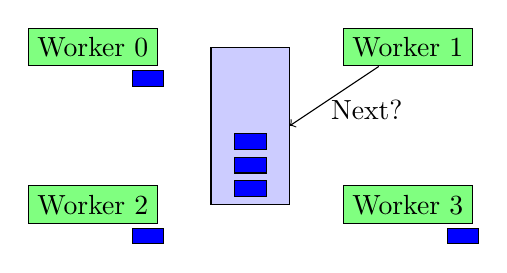
\begin{tikzpicture}
      \node at (0,2) [rectangle,draw=black,fill=green!50] {Worker 0};
      \draw[fill=blue] (0.5,1.7) rectangle (0.9,1.5);
      \node(w1) at (4,2) [rectangle,draw=black,fill=green!50] {Worker 1};
      \draw[->] (w1) -- (2.5,1);
      \node at (2.9,1.2) [right] {Next?};
      \node at (0,0) [rectangle,draw=black,fill=green!50] {Worker 2};
      \draw[fill=blue] (0.5,-0.3) rectangle (0.9,-0.5);
      \node at (4,0) [rectangle,draw=black,fill=green!50] {Worker 3};
      \draw[fill=blue] (4.5,-0.3) rectangle (4.9,-0.5);
      \draw[fill=blue!20,draw=black] (1.5,0) rectangle (2.5,2);
      \draw[fill=blue] (1.8,0.1) rectangle (2.2,0.3);
      \draw[fill=blue] (1.8,0.4) rectangle (2.2,0.6);
      \draw[fill=blue] (1.8,0.7) rectangle (2.2,0.9);
    \end{tikzpicture}
  \end{center}
  
  Idea: obvious parallelization of standard search
  \begin{itemize}
  \item Locks on shared data structure (stack, queue, etc)
  \item Or might be a manager task
  \end{itemize}
\end{frame}

\begin{frame}
  \frametitle{Centralized scheduling}

  Teaser: What could go wrong with this parallel BFS?
  \begin{tabbing}
    \quad \= \quad \= \kill
    Put root in queue \\
    fork \\
    \> obtain queue lock \\
    \> while queue has work \\
    \> \> remove node $n$ from queue \\
    \> \> release queue lock \\
    \> \> process $n$, mark as searched \\
    \> \> obtain queue lock \\
    \> \> enqueue unsearched children of $n$ \\
    \> release queue lock \\
    join
  \end{tabbing}

\end{frame}


\begin{frame}
  \frametitle{Centralized scheduling}

  Teaser: What could go wrong with this parallel BFS?
  \begin{tabbing}
    \quad \= \quad \= \kill
    Put root in queue; {\bf workers active = 0} \\
    fork \\
    \> obtain queue lock \\
    \> while queue has work {\bf or workers active > 0} \\
    \> \> remove node $n$ from queue; {\bf workers active {\tt ++}} \\
    \> \> release queue lock \\
    \> \> process $n$, mark as searched \\
    \> \> obtain queue lock \\
    \> \> enqueue unsearched children of $n$; {\bf workers
      active {\tt --}}\\
    \> release queue lock \\
    join
  \end{tabbing}

\end{frame}


\begin{frame}
  \frametitle{Centralized task queue}

  \begin{itemize}
  \item Called {\em self-scheduling} when applied to loops
    \begin{itemize}
    \item Tasks might be range of loop indices
    \item Assume independent iterations
    \item Loop body has unpredictable time (or do it statically)
    \end{itemize}
  \item Pro: dynamic, online scheduling
  \item Con: centralized, so doesn't scale
  \item Con: high overhead if tasks are small
  \end{itemize}

\end{frame}


\begin{frame}
  \frametitle{Beyond centralized task queue}

  \begin{center}
    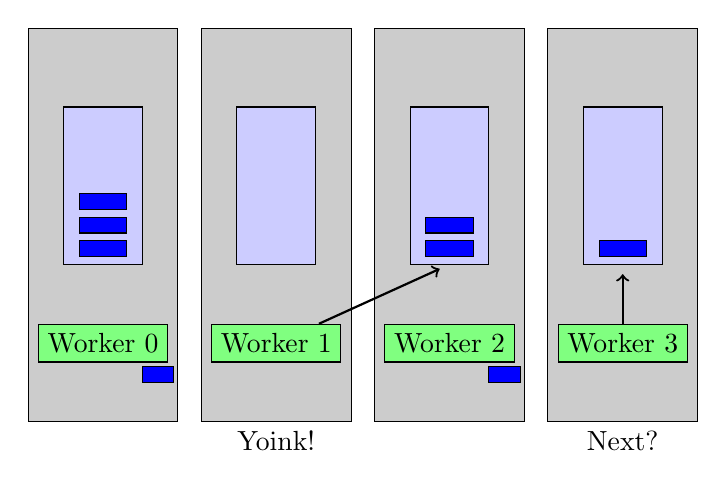
\begin{tikzpicture}
      \begin{scope}
      \node(q0) at (0,1) {};
      \draw[fill=black!20,draw=black] (-0.95,-1) rectangle (0.95,4);
      \draw[fill=blue!20,draw=black] (-0.5,1) rectangle (0.5,3);
      \draw[fill=blue] (-0.3,1.1) rectangle (0.3,1.3);
      \draw[fill=blue] (-0.3,1.4) rectangle (0.3,1.6);
      \draw[fill=blue] (-0.3,1.7) rectangle (0.3,1.9);
      \node(w0) at (0,0) [rectangle,fill=green!50,draw=black] {Worker 0};
      
      \draw[fill=blue] (0.5,-0.3) rectangle (0.9,-0.5);
      \end{scope}

      \begin{scope}[xshift=2.2cm]
      \node(q1) at (0,1) {};        
      \draw[fill=black!20,draw=black] (-0.95,-1) rectangle (0.95,4);
      \draw[fill=blue!20,draw=black] (-0.5,1) rectangle (0.5,3);
      \node (w1) at (0,0) [rectangle,fill=green!50,draw=black] {Worker 1};
      %\draw[fill=blue] (0.5,-0.3) rectangle (0.9,-0.5);
      \end{scope}

      \begin{scope}[xshift=4.4cm]
      \node(q2) at (0,1) {};        
      \draw[fill=black!20,draw=black] (-0.95,-1) rectangle (0.95,4);
      \draw[fill=blue!20,draw=black] (-0.5,1) rectangle (0.5,3);
      \draw[fill=blue] (-0.3,1.1) rectangle (0.3,1.3);
      \draw[fill=blue] (-0.3,1.4) rectangle (0.3,1.6);
      %\draw[fill=blue] (-0.3,1.7) rectangle (0.3,1.9);
      \node(w2) at (0,0) [rectangle,fill=green!50,draw=black] {Worker 2};
      \draw[fill=blue] (0.5,-0.3) rectangle (0.9,-0.5);
      \end{scope}

      \begin{scope}[xshift=6.6cm]
      \node(q3) at (0,1) {};                
      \draw[fill=black!20,draw=black] (-0.95,-1) rectangle (0.95,4);
      \draw[fill=blue!20,draw=black] (-0.5,1) rectangle (0.5,3);
      \draw[fill=blue] (-0.3,1.1) rectangle (0.3,1.3);
      %\draw[fill=blue] (-0.3,1.4) rectangle (0.3,1.6);
      %\draw[fill=blue] (-0.3,1.7) rectangle (0.3,1.9);
      \node(w3) at (0,0) [rectangle,fill=green!50,draw=black] {Worker 3};
      %\draw[fill=blue] (0.5,-0.3) rectangle (0.9,-0.5);
      \end{scope}

      \draw[thick,->] (w1) -- (q2);
      \draw[thick,->] (w3) -- (q3);
      \node at (2.2,-1) [below] {Yoink!};
      \node at (6.6,-1) [below] {Next?};
    \end{tikzpicture}
  \end{center}
\end{frame}

\begin{frame}
  \frametitle{Beyond centralized task queue}
  
  Basic {\em distributed} task queue idea:
  \begin{itemize}
  \item Each processor works on part of a tree
  \item When done, get work from a peer
  \item {\em Or} if busy, push work to a peer
  \item Requires asynch communication
  \end{itemize}
  Also goes by work stealing, work crews...
  
  \vspace{5mm}
  Implemented in OpenMP, Cilk, X10, CUDA, QUARK, SMPss, ...
\end{frame}


\begin{frame}
  \frametitle{Picking a donor}

  Could use:
  \begin{itemize}
  \item Asynchronous round-robin
  \item Global round-robin (keep current donor pointer at proc 0)
  \item Randomized -- optimal with high probability!
  \end{itemize}

\end{frame}


\begin{frame}
  \frametitle{Diffusion-based balancing}

  \begin{itemize}
  \item Problem with random polling: communication cost!
    \begin{itemize}
    \item But not all connections are equal
    \item Idea: prefer to poll more local neighbors
    \end{itemize}
  \item Average out load with neighbors $\implies$ diffusion!
  \end{itemize}
\end{frame}


\begin{frame}
  \frametitle{Mixed parallelism}

  \begin{itemize}
  \item Today: mostly coarse-grain {\em task} parallelism
  \item Other times: fine-grain {\em data} parallelism
  \item Why not do both?  {\em Switched} parallelism.
  \end{itemize}
\end{frame}


\begin{frame}
  \frametitle{Takeaway}

  \begin{itemize}
  \item Lots of ideas, not one size fits all!
  \item Axes: task size, task dependence, communication
  \item Dynamic tree search is a particularly hard case!
  \item Fundamental tradeoffs
    \begin{itemize}
    \item Overdecompose (load balance) vs \\
      keep tasks big (overhead, locality)
    \item Steal work globally (balance) vs \\
      steal from neighbors (comm.~overhead)
    \end{itemize}
  \item Sometimes hard to know when code should stop!
  \end{itemize}
\end{frame}


\end{document}
